
\documentclass[a4paper,12pt]{article}
\usepackage[utf8]{inputenc}
\usepackage[serbian]{babel}
\usepackage{amsmath,amsfonts,amssymb}
\usepackage{graphicx}

\begin{document}

\section*{Zadaci oblast 1}

\subsection*{Zadatak 1}
Godina je prestupna ako zadovoljava sledeće osnovne uslove:
\begin{enumerate}
    \item deljiva je sa 4 i nije deljiva sa 100,
    \item deljiva je sa 400.
\end{enumerate}

Koliko ima prestupnih godina u intervalu godina $[1501, 2501]$?

Rešenje:

Neka je $A$ skup godina deljivih sa 4 koje nisu deljive sa 100 i neka je $B$ skup godina deljivih sa 400, sve u periodu između 1501. i 2501. godine. Ako je godina deljiva sa 400, onda je ona deljiva i sa 100, što znači da je $A \cap B = \emptyset$. Tada je broj prestupnih godina u periodu između 1501. i 2501. godine jednak:
\[
|A \cup B| = |A| + |B|.
\]

Broj godina između 1501. i 2501. godine koje su deljive sa 4, a nisu deljive sa 100, jednak je:
\[
|A| = 250 - 10 = 240.
\]
Skup godina između 1501. i 2501. godine koje su deljive sa 400 jednak je:
\[
|B| = 3.
\]

Znači, ukupno ima $243$ prestupne godine.


\subsection*{Zadatak 2}
Odrediti koliko ima petocifrenih brojeva:
\begin{enumerate}
    \item ukupno,
    \item čije su cifre svi parni brojevi,
    \item čije su cifre svi neparni brojevi,
    \item čija bar jedna cifra je neparan broj,
    \item čija bar jedna cifra je paran broj,
    \item čija bar jedna cifra je paran broj i bar jedna cifra je neparan broj.
\end{enumerate}

Rešenje:

Neka je:
\begin{align*}
    A &= \{x \in \mathbb{N} : x \text{ je petocifren broj}\}, \\
    B &= \{x \in A : x \text{ ima sve parne cifre}\}, \\
    C &= \{x \in A : x \text{ ima sve neparne cifre}\}, \\
    D &= \{x \in A : x \text{ ima bar jednu parnu cifru}\}, \\
    E &= \{x \in A : x \text{ ima bar jednu neparnu cifru}\}, \\
    F &= \{x \in A : x \text{ ima bar jednu parnu i bar jednu neparnu cifru}\}.
\end{align*}

U svim slučajevima, koristimo oznaku \(A_1, \ldots, A_5\) za skup cifara koje mogu biti na poziciji \(i\).  
Petocifrene brojeve možemo predstaviti kao uređene petorke iz skupa:
\[
A_1 \times A_2 \times A_3 \times A_4 \times A_5,
\]
gde se ti skupovi razlikuju od slučaja do slučaja.

(i) Ukupno
Ako prva cifra ne može biti 0:
\[
A_1 = \{1, 2, 3, 4, 5, 6, 7, 8, 9\}, \quad A_2 = A_3 = A_4 = A_5 = \{0, 1, 2, 3, 4, 5, 6, 7, 8, 9\}.
\]
Na osnovu principa proizvoda:
\[
|A| = |A_1| \cdot |A_2| \cdot |A_3| \cdot |A_4| \cdot |A_5| = 9 \cdot 10 \cdot 10 \cdot 10 \cdot 10 = 90000.
\]

(ii) Svi parni brojevi
Ako sve cifre moraju biti parne:
\[
A_1 = \{2, 4, 6, 8\}, \quad A_2 = A_3 = A_4 = A_5 = \{0, 2, 4, 6, 8\}.
\]
Na osnovu principa proizvoda:
\[
|B| = |A_1| \cdot |A_2| \cdot |A_3| \cdot |A_4| \cdot |A_5| = 4 \cdot 5 \cdot 5 \cdot 5 \cdot 5 = 2500.
\]

(iii) Svi neparni brojevi
Ako sve cifre moraju biti neparne:
\[
A_1 = A_2 = A_3 = A_4 = A_5 = \{1, 3, 5, 7, 9\}.
\]
Na osnovu principa proizvoda:
\[
|C| = |A_1| \cdot |A_2| \cdot |A_3| \cdot |A_4| \cdot |A_5| = 5^5 = 3125.
\]

(iv) Bar jedna parna cifra
Može se primetiti da je \(A = B \cup D \cap E = \emptyset\).  
Tada je na osnovu principa zbira:
\[
|D| = |A| - |B| = 90000 - 2500 = 87500.
\]

(v) Bar jedna neparna cifra
Slično kao u prethodnom slučaju, važi da \(A = C \cup E\) i \(C \cap E = 0\).  
Na osnovu principa zbira:
\[
|E| = |A| - |C| = 90000 - 3125 = 86875.
\]

(vi) Bar jedna parna i bar jedna neparna cifra
Prema principu uključivanja-isključivanja:
\[
|F| = |D| + |E| - |A| = 87500 + 86875 - 90000 = 84375.
\]

\subsection*{Zadatak 3}
Koliko se najviše kraljeva može postaviti na šahovsku tablu dimenzije \(8 \times 8\), tako da se oni međusobno ne napadaju?

Rešenje:

Moguće je postaviti 16 kraljeva i jedan od mogućih rasporeda je prikazan na slici levo (dovoljno je pronaći jedan takav raspored).  
Pretpostavimo sada da je moguće rasporediti više od 16 kraljeva. Ako podelimo tablu na 16 delova dimenzija \(2 \times 2\):

\begin{center}
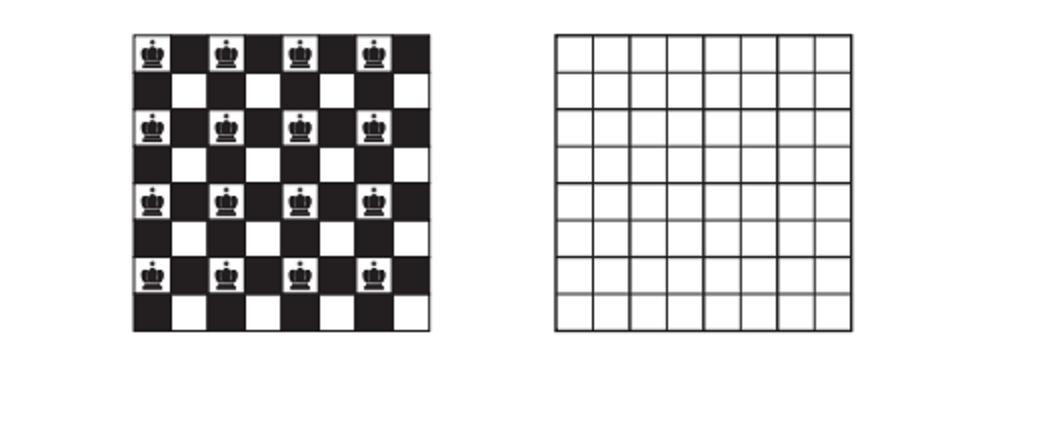
\includegraphics[width=0.4\textwidth]{sahovska_tabla.png}
\end{center}

onda bi se, zbog Dirihleovog principa, u jednom delu morala nalaziti bar 2 kralja. Međutim, zbog načina na koji se kreće po šahovskoj tabli ova dva kralja se uvek napadaju, te je maksimalan broj kraljeva koji se mogu rasporediti na tabli 16.


\end{document}
